%% The following is a directive for TeXShop to indicate the main file
%%!TEX root = diss.tex

\chapter{Materials and Methods}
\label{ch:Materialsandmethods}

%%%%%%%%%%%%%%%%%%%%%%%%%%%%%%%%%%%%%%%%%%%%%%%%%%%%%%%%%%%%%%%%%%%%%%
\section{Overview of study design}
\label{sec:Overviewofstudydesign}

This study involved retrospective analysis of amplicon-based targeted sequencing data from 213 cancer patients with FFPE tumour and matched blood specimens. Extracted DNA from specimens were sheared, enriched for amplicons in the OncoPanel, barcoded, and subjected to next-generation sequencing. Sequencing data were processed and analyzed with a custom variant-calling pipeline. To verify that FFPE DNA is a reliable resource for germline testing, we assessed the degree of formalin-induced DNA damages in FFPE specimens by comparing the efficiency in amplicon enrichment and sequencing results of FFPE specimens to blood. We applied a bioinformatics approach in discriminating between germline and somatic statuses of variants in FFPE tumours, and we calculated the true positive rate for detection of germline variants in FFPE tumours. Because the tumour genome contains germline and somatic variants, potential germline variants detected using tumour sequencing must be confirmed with downstream germline testing. Hence, we established a balance between true positive rate for detection of germline variants in FFPE tumours and positive predictive value for referral of potential germline variants for downstream confirmatory testing.

%%%%%%%%%%%%%%%%%%%%%%%%%%%%%%%%%%%%%%%%%%%%%%%%%%%%%%%%%%%%%%%%%%%%%%
\section{Patient samples}
\label{sec:Patientsamples}

Blood and FFPE tumour specimens were acquired from 213 patients who provided informed consent for The OncoPanel Pilot (TOP) study, a pilot study to optimize the OncoPanel, which is an amplicon-based targeted NGS panel for solid tumours. The TOP study also aims to assess the OncoPanel's application for guiding disease management and therapeutic intervention. Patients in the TOP study are those with advanced cancers including colorectal cancer, lung cancer, melanoma, gastrointestinal stromal tumour (GIST), and other cancers (\autoref{tbl:cancertypes}). The age of paraffin block for tumour specimens ranges from 18 to 5356 days with a median of 274 days.

\begin{table}[H]
\caption{Distribution of cancer types in the TOP cohort.}
\label{tbl:cancertypes}
\centering
      \begin{tabular}{lccc}
        \hline
        Cancer Type & Number of Cases & Percentage (\%) \\ \hline
        Colorectal & 97 & 46 \\
        Lung & 59 & 28 \\
        Melanoma & 18 & 8 \\
				Other\textsuperscript{$\dagger$} & 17 & 8 \\
				GIST & 7 & 3 \\
				Sarcoma & 4 & 2 \\
				Neuroendocrine & 4 & 2 \\
				Cervical & 2 & 0.9 \\
				Ovarian & 2 & 0.9 \\
				Breast & 2 & 0.9 \\
				Unknown & 1 & 0.5 \\ \hline
      \end{tabular} \\
			\vspace{0.5cm}
\justify
{\small \textsuperscript{$\dagger$}This category includes thyroid, peritoneum, lung sarcomatoid carcinoma, Fallopian tube, gastric, endometrial, squamous cell carcinoma, anal, salivary gland, peritoneal epithelial mesothelioma, adenoid cystic carcinoma, pancreas, breast, gall bladder, parotid epithelial myoepithelial carcinoma, and small bowel cancers.}
\end{table}

%%%%%%%%%%%%%%%%%%%%%%%%%%%%%%%%%%%%%%%%%%%%%%%%%%%%%%%%%%%%%%%%%%%%%%
\section{Sample preparation, library construction, and Illumina sequencing}
\label{sec:Samplepreparation,libraryconstruction,andIlluminasequencing}

Genomic DNA was extracted from blood and FFPE tumour specimens using the Gentra Autopure LS DNA preparation platform and QIAamp DNA FFPE tissue kit (Qiagen, Hilden, Germany), respectively. The extracted DNA was sheared according to a previously described protocol \cite{Bosdet2013} to attain approximate sizes of 3 kb followed by PCR primer merging, amplification of target regions, and adapter ligation using the Thunderstorm NGS Targeted Enrichment System (RainDance Technologies, Lexington, MA) as per manufacturer's protocol. Barcoded amplicons were sequenced with the Illumina MiSeq system for paired end sequencing with a v2 250-bp kit (Illumina, San Diego, CA).


%%%%%%%%%%%%%%%%%%%%%%%%%%%%%%%%%%%%%%%%%%%%%%%%%%%%%%%%%%%%%%%%%%%%%
\section{OncoPanel (Amplicon-based targeted sequencing panel for solid tumours)}
\label{sec:OncoPanel}

The OncoPanel assesses coding exons and clinically relevant hotpots of 15 cancer predisposing genes and six PGx genes that can predict chemotherapeutic response. Primers were designed by RainDance Technologies (Lexington, MA) using the GRCh37/hg19 reference sequence to generate 416 amplicons between 56 bp and 288 bp in size, which interrogate $\sim$ 20 kb of target bases. Complete list of genes and gene reference models for the OncoPanel is presented in \autoref{tbl:genemodel}, whereas OncoPanel target regions and amplicons are presented in \autoref{tbl:amplicons_target_regions}.

\normalsize
\begin{table}[H]
    \caption{Gene reference models for HGVS nomenclature.}
    \label{tbl:genemodel}
    \centering
    \begin{tabular}{llll}
    \hline
    Gene & Protein & Reference Model \\
    \hline
    \multicolumn{3}{l}{\textit{Cancer-causing}}
    \\
    AKT1 & Protein kinase B & NM\_001014431.1 \\
    ALK & Anaplastic lymphoma receptor tyrosine kinase & NM\_004304.3 \\
    BRAF & Serine/threonine-protein kinase B-Raf & NM\_004333.4 \\
    EGFR & Epidermal growth factor receptor & NM\_005228.3 \\
    HRAS & GTPase HRas & NM\_005343.2 \\
    MAPK1 & Mitogen-activated protein kinase 1 & NM\_002745.4 \\
    MAP2K1 & Mitogen-activated protein kinase kinase 1 & NM\_002755.3 \\
    MTOR & Serine/threonine-protein kinase mTOR & NM\_004958.3 \\
    NRAS & Neuroblastoma RAS viral oncogene homolog & NM\_002524.3 \\
    PDGFRA & Platelet-derived growth factor receptor alpha & NM\_006206.4 \\
    PIK3CA & Phosphatidylinositol-4,5-bisphosphate 3-kinase catalytic subunit alpha & NM\_006218.2 \\
    PTEN & Phosphatase and tensin homolog & NM\_000314.4 \\
    STAT1 & Signal transducer and activator of transcription 1 & NM\_007315.3 \\
    STAT3 & Signal transducer and activator of transcription 3 & NM\_139276.2 \\
    TP53 & Tumor protein P53 & NM\_000546.5 \\
    \\
    \multicolumn{3}{l}{\textit{Pharmacogenomics}}
    \\
    DPYD & Dihydropyrimidine dehydrogenase & NM\_000110.3 \\
    GSTP1 & Glutathione S-rransferase pi 1 & NM\_000852.3 \\
    MTHFR & Methylenetetrahydrofolate reductase & NM\_005957.4 \\
    TYMP & Thymidine phosphorylase & NM\_001113755.2 \\
    TYMS & Thymidylate synthetase & NM\_001071.2 \\
    UGT1A1 & Uridine diphosphate (UDP)-glucuronosyl transferase 1A1 & NM\_000463.2\\
    \hline
    \end{tabular}
\end{table}


%%%%%%%%%%%%%%%%%%%%%%%%%%%%%%%%%%%%%%%%%%%%%%%%%%%%%%%%%%%%%%%%%%%%%%
\section{Variant calling pipeline}
\label{sec:Variantcallingpipeline}

\subsection{Read alignment and variant calling}

Reads that passed the Illumina Chastity filter were aligned to the GRCh37/hg19 human reference genome using the BWA mem algorithm (version 0.5.9) with default parameters, and the alignments were processed and converted to the BAM format using SAMtools (version 0.1.18). The SAMtools \texttt{mpileup} function \texttt{(samtools mpileup -BA -d 500000 -L 500000 -q 1)} was used to generate pileup files for all target bases followed by variant calling with the VarScan2 \texttt{mpileup2cns} (version 2.3.6) function with parameter thresholds of variant allele frequency $\geq$ 10\% and Phred-scaled base quality score $\geq$ 20 \texttt{(--min-var-freq 0.1 --p-value 0.01 --strand-filter 0 --output-vcf --variants --min-avg-qual 20)}.

\subsection{Variant filtering}

Variant calls were filtered using the VarScan2 \texttt{fpfilter} function with fraction of variant reads from each strand $\geq$ 0.1 and default thresholds for other parameters (\autoref{tbl:varscan_fpfilter_parameters}). The VarScan2 \texttt{fpfilter} removed 257 low quality variants. Eighty out of the 257 variants were germline variants detected in blood, but filtered out from FFPE specimens by the VarScan2 \texttt{fpfilter}. Thus, these eighty calls were excluded from further analysis as well. Manual inspection was performed for a subset of variants, including variants detected within primer regions and in PGx genes, using the Intergrative Genomics Viewer (IGV, version 2.3). This resulted in the removal of 500 spurious calls, which stemmed from software bugs, sequencing artifacts, primer masking, and primer artifacts (\autoref{tbl:spurious_calls}). Twelve low coverage calls ($\leq$ 100x) were also excluded. Implementation of this filtering pipeline reduced the raw variant output of 6169 calls from 217 tumour-blood paired samples (434 sequencing libraries) to 5320 calls (\autoref{fig:variant_pipeline}B).

\subsection{Variant annotation and interpretation}

SnpEff (version 4.2) was used for variant annotation and effect prediction, and the SnpSift package in SnpEff was used to annotate variants with databases such as dbSNP (b138), COSMIC (version 70), 1000 Genomes Project, and ExAC (release 0.3) for interpretation. Clinical significance reported by the ClinVar database was also used for variant interpretation.


%%%%%%%%%%%%%%%%%%%%%%%%%%%%%%%%%%%%%%%%%%%%%%%%%%%%%%%%%%%%%%%%%%%%%%
%%%%%%%%%%%%%%%%%%%%%%%%%%%%%%%%%%%%%%%%%%%%%%%%%%%%%%%%%%%%%%%%%%%%%%

\begin{table}[H]
\caption{Thresholds for parameters of VarScan2 \texttt{fpfilter} used for filtering raw variant output.}
\label{tbl:varscan_fpfilter_parameters}
\centering
      \begin{tabular}{p{0.3\linewidth}p{0.56\linewidth}cp{0.1\linewidth}}
        \hline
        Parameter & Description & Threshold
				\\
				\hline
				\texttt{--min-var-count} & Min number of var-supporting reads & 4
				\\
        \texttt{--min-var-count-lc} & Min number of var-supporting reads when depth below somaticPdepth & 2
        \\
        \texttt{--min-var-freq} & Min variant allele frequency & 0.1
				\\
        \texttt{--max-somatic-p} & Max somatic p-value & 0.05
				\\
        \texttt{--max-somatic-p-depth} & Depth required to test max somatic p-value & 10
				\\
        \texttt{--min-ref-readpos} & Min average read position of ref-supporting reads & 0.1
				\\
        \texttt{--min-var-readpos} & Min average read position of var-supporting reads & 0.1
				\\
        \texttt{--min-ref-dist3} & Min average distance to effective 3' end of ref reads & 0.1
				\\
        \texttt{--min-var-dist3} & Min average distance to effective 3' end of variant reads & 0.1
				\\
        \texttt{--min-strandedness} & Min fraction of variant reads from each strand & 0.1
				\\
        \texttt{--min-strand-reads} & Min allele depth required to perform the strand tests & 5
				\\
        \texttt{--min-ref-basequal} & Min average base quality for ref allele & 15
				\\
        \texttt{--min-var-basequal} & Min average base quality for var allele & 15
				\\
        \texttt{--min-ref-avgrl} & Min average trimmed read length for ref allele & 90
				\\
        \texttt{--min-var-avgrl} & Min average trimmed read length for var allele & 90
        \\
        \texttt{--max-rl-diff} & Max average relative read length difference (ref - var) & 0.25
        \\
        \texttt{--max-ref-mmqs} & Max mismatch quality sum of ref-supporting reads & 100
        \\
        \texttt{--max-var-mmqs} & Max mismatch quality sum of var-supporting reads & 100
        \\
        \texttt{--max-mmqs-diff} & Max average mismatch quality sum (var - ref) & 50
        \\
        \texttt{--min-ref-mapqual} & Min average mapping quality for ref allele & 15
        \\
        \texttt{--min-var-mapqual} & Min average mapping quality for var allele & 15
        \\
        \texttt{--max-mapqual-diff} & Max average mapping quality (ref - var) & 50
        \\
				\hline
      \end{tabular}
\end{table}

%%%%%%%%%%%%%%%%%%%%%%%%%%%%%%%%%%%%%%%%%%%%%%%%%%%%%%%%%%%%%%%%%%%%%%
%%%%%%%%%%%%%%%%%%%%%%%%%%%%%%%%%%%%%%%%%%%%%%%%%%%%%%%%%%%%%%%%%%%%%%

\begin{table}[H]
\caption{Spurious variants removed by the variant filtering pipeline.}
\label{tbl:spurious_calls}
\centering
      \begin{tabular}{lllllll}
        \hline
        Gene & Chr & Pos & Ref & Alt & Reason
				\\
				\hline
				KIT & chr4 & 55599268 & C & T & Variant masked by primer in FFPE specimen
				\\
        MAPK1 & chr22 & 22162126 & A & G & Variant masked by primer in FFPE specimen
        \\
        MTOR & chr1 & 11186783 & G & A & Sequencing artifact within primer region
        \\
        MTOR & chr1 & 11190646 & G & A & Variant masked by primer in FFPE specimen
        \\
        TYMP & chr22 & 50964446 & A & T & Poor target region, alignment of different sized amplicons
        \\
        TYMP & chr22 & 50964862 & A & T & Poor target region, alignment of different sized amplicons
        \\
        TYMS & chr18 & 673449 & G & C & VarScan2 bug after chr18:673443 c.*447\_*452delTTAAAG
        \\
        UGT1A1 & chr2 & 234668879 & CAT & C & Sequencing artifact at AT repeats in promoter
        \\
        UGT1A1 & chr2 & 234668881 & T & TAC & VarScan2 bug after AT insertion in promoter
        \\
				\hline
      \end{tabular}
\end{table}

%%%%%%%%%%%%%%%%%%%%%%%%%%%%%%%%%%%%%%%%%%%%%%%%%%%%%%%%%%%%%%%%%%%%%%
%%%%%%%%%%%%%%%%%%%%%%%%%%%%%%%%%%%%%%%%%%%%%%%%%%%%%%%%%%%%%%%%%%%%%%

\begin{figure}[H]
\centering
	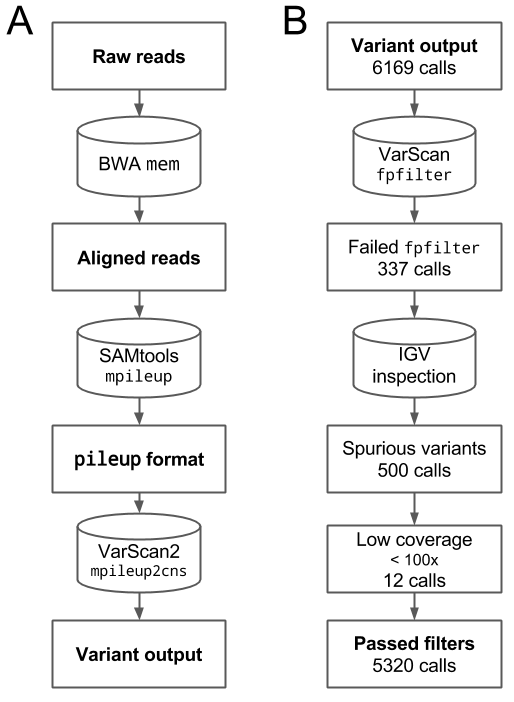
\includegraphics[scale=0.55]{variant_pipeline2.png}
	\caption{Pipelines for (A) variant calling and (B) filtering.}
	\label{fig:variant_pipeline}
\end{figure}

%%%%%%%%%%%%%%%%%%%%%%%%%%%%%%%%%%%%%%%%%%%%%%%%%%%%%%%%%%%%%%%%%%%%%%
\section{Sequence analysis}
\label{sec:Sequenceanalysis}

Coverage depth was measured using bedtools (version 2.25.0) and per-base metrics were obtained using bam-readcount (https://github.com/genome/). Statistical analyses and data visualization were performed using R (version 3.3.2) and associated open-source packages. Manual review of PGx variants were carried out using the Intergrative Genomics Viewer (IGV, version 2.3). \textit{Note: be more specific on how the data is generated}

%%%%%%%%%%%%%%%%%%%%%%%%%%%%%%%%%%%%%%%%%%%%%%%%%%%%%%%%%%%%%%%%%%%%%%
\section{Bioinformatics approaches for identification of germline variants in FFPE tumours}
\label{sec:BioinformaticsapproachesforidentificationofgermlinevariantsinFFPEtumours}

%%%%%%%%%%%%%%%%%%%%%%%%%%%%%%%%%%%%%%%%%%%%%%%%%%%%%%%%%%%%%%%%%%%%%%
%%%%%%%%%%%%%%%%%%%%%%%%%%%%%%%%%%%%%%%%%%%%%%%%%%%%%%%%%%%%%%%%%%%%%%

\begin{figure}[H]
\centering
	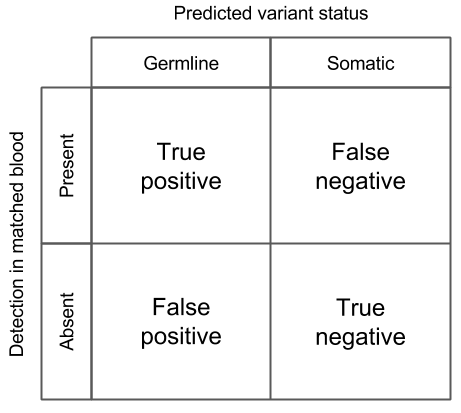
\includegraphics[scale=0.55]{tpfptnfn.png}
	\caption{Determination of true positives, false positives, true negatives, and false negatives from variant calls.}
	\label{fig:tpfptnfn}
\end{figure}


%%%%%%%%%%%%%%%%%%%%%%%%%%%%%%%%%%%%%%%%%%%%%%%%%%%%%%%%%%%%%%%%%%%%%%

\endinput
